% !TeX root = ../main.tex

\chapter{移植记录}

\section{搭建开发环境}

310b\_rc\_24.1.rc2\_5.0.3 支持由源码编译，进行源码编译前，请根据如下步骤完成相关环境准备。

\subsection{硬件环境}

准备一台 X86 架构、预装 Ubuntu 系统的设备，硬盘容量不小于 200GB。

\subsection{安装库和工具集}

可参考官方相关链接\hyperref[ref:oh-build]{[3]}；这里以 Ubuntu 22.04 为例：

\subsubsection{安装基础依赖}

\begin{lstlisting}[style=shell, caption={安装基础依赖}]
#安装基础依赖
sudo apt update
sudo apt upgrade
sudo apt install -y \
  openjdk-11-jdk \
  ccache \
  libelf-dev \
  dwarves \
  genext2fs \
  u-boot-tools \
  mtools \
  mtd-utils \
  scons \
  gcc-arm-none-eabi \
  build-essential \
  ninja-build \
  ruby \
  git \
  curl \
  unzip \
  python3 \
  python3-pip \
  bc \
  flex \
  bison \
  libssl-dev
\end{lstlisting}

\subsubsection{安装编译工具}

\begin{lstlisting}[style=shell, caption={安装编译工具}]
#安装编译工具
sudo apt-get update
sudo apt-get install build-essential
sudo apt-get install libncurses*
sudo apt-get install lzop
sudo apt-get install net-tools
sudo apt-get install openssh-server vim git fakeroot
\end{lstlisting}

\subsubsection{安装扩展依赖}

\begin{lstlisting}[style=shell, caption={安装扩展依赖}]
#安装扩展依赖
sudo apt-get install git ssh make gcc libssl-dev liblz4-tool expect \
  g++ patchelf chrpath gawk texinfo chrpath diffstat binfmt-support \
  qemu-user-static live-build bison flex fakeroot cmake gcc-multilib \
  g++-multilib unzip device-tree-compiler python3-pip libncurses5-dev
sudo apt-get install libgmp-dev libmpc-dev libicu-dev bsdmainutils
sudo apt-get -y apt-utils binutils bison flex bc build-essential make \
  mtd-utils gcc-arm-linux-gnueabi u-boot-tools python3-pip git zip \
  unzip curl wg
\end{lstlisting}

\subsection{配置 git 账户信息}

\begin{lstlisting}[style=shell, caption={Git 配置}]
#Git配置
git config --global user.name "HFUT_QDZDD"
git config --global user.email "example@mail.hfut.edu.cn"
git config --global credential.helper store
ssh-keygen -t ed25519 -C "Gitcode SSH Key"
\end{lstlisting}

\subsection{安装码云 repo 工具}

\begin{lstlisting}[style=shell, caption={安装 Repo}]
#安装Repo
mkdir ~/bin
curl https://raw.gitcode.com/gitcode-dev/repo/raw/main/repo-py3 -o ~/bin/repo
chmod a+x ~/bin/repo
pip3 install -i https://repo.huaweicloud.com/repository/pypi/simple requests
#将repo添加到环境变量
vim ~/.bashrc
export PATH=~/bin:$PATH
source ~/.bashrc
\end{lstlisting}

\subsection{安装内核交叉编译工具链}

复制 Ascend-hdk-310b-sdk-soc\_24.1.rc2.zip Ascend HDK 24.1.RC2 中的 toolchain.tar.gz 至 /opt，并解压。

\begin{lstlisting}[style=shell, caption={配置工具链}]
#配置工具链
sudo mkdir /opt/compiler
sudo sh -c 'echo "export PATH=/opt/compiler/toolchain/bin:\$PATH" >> /etc/profile'
source /etc/profile
cp toolchain/ /opt/compiler/ -rf
\end{lstlisting}


\section{源码下载}

执行如下命令，下载 310b\_rc\_24.1.rc2\_5.0.3 仓源码：通过 repo + ssh 下载（需注册公钥，请参考码云帮助中心\hyperref[ref:gitee-help]{[4]}）。

\subsection{从版本分支获取源码}

可获取该版本分支的最新源码，包括版本发布后在该分支的合入（后文称该分支为动态分支）。

\begin{lstlisting}[style=shell, caption={下载分支源码}]
#下载分支源码
export REPO_URL='https://mirrors.tuna.tsinghua.edu.cn/git/git-repo'
repo init -u git@gitee.com:openharmony/manifest.git \
  -b OpenHarmony-5.0.3-Release --no-repo-verify
repo sync -c
repo forall -c 'git lfs pull'
\end{lstlisting}

\noindent\textbf{PS. 网络问题解决方案：}清理已下载但不完整的仓库，重新单线程同步。

\subsection{从版本发布的 Tag 节点获取源码}

可获取与版本发布时完全一致的源码（后文称该分支为发布分支，该分支问题较多，不建议使用）。

\begin{lstlisting}[style=shell, caption={下载 Tag 源码}]
#下载Tag源码
repo init -u git@gitee.com:openharmony/manifest.git \
  -b refs/tags/OpenHarmony-v5.0.3-Release --no-repo-verify
repo sync -c
repo forall -c 'git lfs pull'
\end{lstlisting}

\subsection{预编译文件下载}

\begin{lstlisting}[style=shell, caption={下载预编译文件}]
#先进入源码目录，然后下载预编译文件
cd ./build
sudo ./prebuilts_download.sh
\end{lstlisting}

\section{额外厂家源码下载与替换}

\begin{itemize}
  \item 下载 package/Ascend-hdk-310b-npu-driver-soc\_24.1.rc2\_linux-aarch64.run 文件\hyperref[ref:npu-driver]{[18]}。
  \item 下载 package/Ascend310B-source-bjjc-ohos.tar.gz 文件（脚本可能执行失败，要根据报错手动解压）\hyperref[ref:ascend310b-src]{[19]}。
  \item 下载 device\_board\_ascend/ascend/310B/ascendinstall/libaarch64.tar.gz 文件\hyperref[ref:libaarch64]{[20]}。
\end{itemize}


\section{编译制作镜像}

\subsection{权限添加}

执行以下命令添加执行权限：

\begin{lstlisting}[style=shell, caption={添加执行权限}]
chmod +x ./device/board/ascend/310B/kernel/build_kernel.sh
chmod +x ./device/board/ascend/310B/kernel/make-ohos.sh
\end{lstlisting}

\subsection{编译}

厂家已经提供一键式编译安装能力，进入本源码仓代码根目录，执行 build.sh，后面跟 OpenHarmony 源码根目录，这里以/opt/ohos 举例：

\begin{lstlisting}[style=shell, caption={一键编译}]
#一键编译
sudo ./build.sh /opt/ohos
\end{lstlisting}

编译完成后会在 \texttt{/opt/ohos/out/310B/packages/phone/images} 目录下生成 \texttt{Ascend-hdk-310b-soc\_24.1.rc2-harmony\_5.0.3-aarch64.zip} 包。

\noindent\textbf{PS. 编译失败补丁：}可能需要打入下面的 patch：

\begin{lstlisting}[style=shell, caption={编译失败补丁}]
https://gitee.com/phytium_embedded/phytium-openharmony-device/blob/5.x_release/device_board_phytium/common/patch/0032=foundation-arkui-napi=fix_libjsvm_may_compile_fail.patch
\end{lstlisting}

为了减少每次编译时都要设置环境变量，可以在 build.sh 中添加环境配置：

\begin{lstlisting}[style=shell, caption={环境配置}]
echo "export PATH=/opt/compiler/toolchain/bin:\$PATH: " >> /etc/profile
source /etc/profile
\end{lstlisting}

\subsection{动态分支的编译问题修复}

\begin{itemize}
  \item \path{0042=foundation-multimedia-image_effect=fix-egl-function-by-eglGetProcAddress} 补丁失败，请手动添加（行数不对应）。0042 补丁已提交为 \path{task1_transplantation/patch_fix/foundation-multimedia-image_effect-frameworks-native-render_environment-graphic-gl_utils.cpp.patch}。
  \end{itemize}

\subsection{Tag 快照编译的问题修复}

\begin{itemize}
  \item \path{0042=foundation-multimedia-image_effect=fix-egl-function-by-eglGetProcAddress} 补丁失败，请手动添加（行数不对应）。0042 补丁已提交为 \path{task1_transplantation/patch_fix/foundation-multimedia-image_effect-frameworks-native-render_environment-graphic-gl_utils.cpp.patch}。
  \item \textbf{jsvm 语法错误：} \path{5.0.3/foundation/arkui/napi/jsvm/build_jsvm_inter.sh: 行 157}。修复：在 \texttt{"true"} 后面打一个空格。
  \item \textbf{参数错误：} \path{base/hiviewdfx/hiview/plugins/eventlogger/log_catcher/peer_binder_catcher.cpp:408}。修复：\texttt{DoExecHiperf(fileName, pids, processId, perfCmd)} 删除后面两个参数。
  \item \textbf{参数错误：} \path{/foundation/window/window_manager/window_scene/session_manager/src/scene_session_manager.cpp:2396 行}。修复：去除一个参数。
\end{itemize}

\subsection{镜像制作}

下载制卡工程 device\_board\_ascend/310BFormatTest 到 Ubuntu 环境，根据README指示，复制相关库到/usr/lib64/目录下。将编译生成镜像 Ascend-hdk-310b-soc\_24.1.rc2-harmony\_5.0.3-aarch64.zip 解压到 310BFormatTest/firmware。将 SD 卡连上虚拟机或者服务器，执行如下命令：

\begin{lstlisting}[style=shell, caption={制卡命令}]
#复制相关库，添加权限
cp tools/library/* /usr/lib64/
chmod 777 tools/emmc-head

#安装arm64交叉编译 C 标准库
sudo apt install -y libc6-dev-arm64-cross

#制卡命令
cd 310BFormatTest
./formatSD310B.sh /dev/sdX
\end{lstlisting}


\section{编译和烧录}

以上步骤完成后，之后的编译可参考提交的 \texttt{scripts/build\_and\_flash\_310B.sh} 脚本进行一键编译和烧录。

如果修改了内核的相关配置，编译前请删除out目录，再进行编译，否则可能修改不生效。

\section{系统启动与桌面展示}

\begin{figure}[htbp]
  \centering
  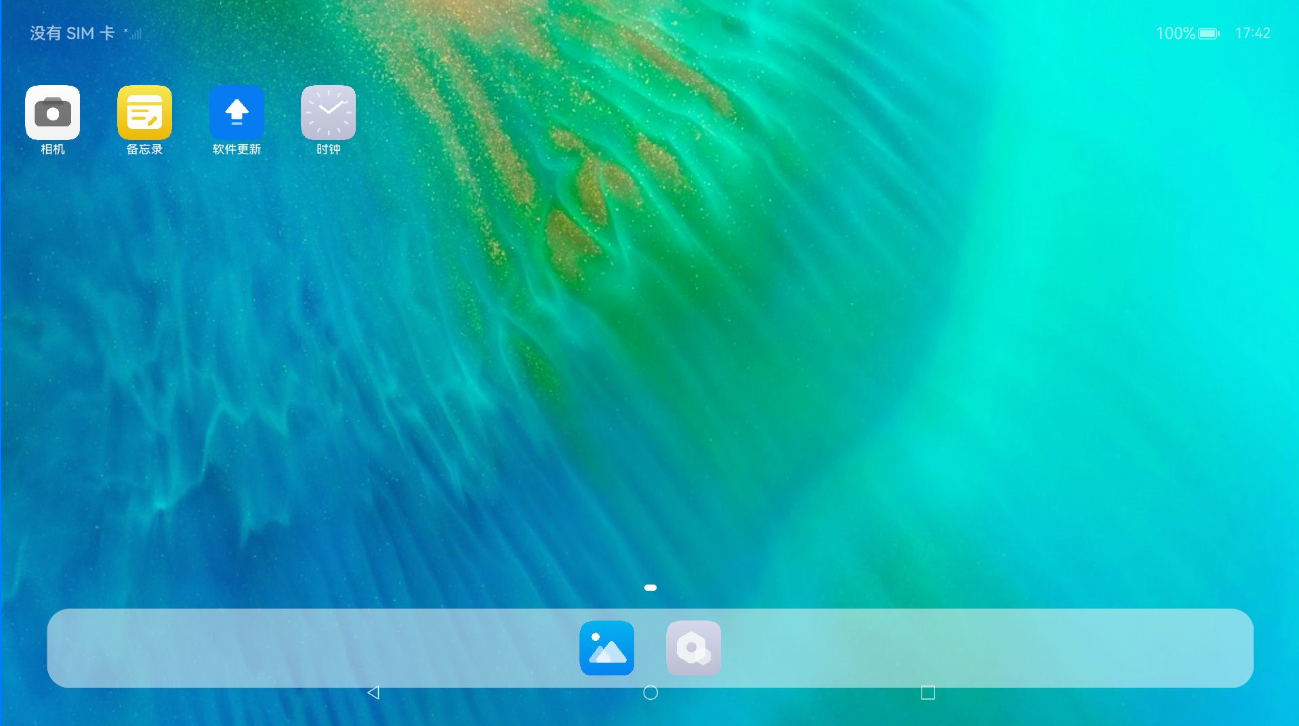
\includegraphics[width=0.8\textwidth]{Desktop.png}
  \caption{桌面展示}
  \label{fig:Desktop}
\end{figure}

\begin{figure}[htbp]
  \centering
  \includegraphics[width=0.8\textwidth]{1080P.png}
  \caption{分辨率展示}
  \label{fig:1080P}
\end{figure}